\thispagestyle{duongvaotoanhocnone}
\pagestyle{duongvaotoanhoc}
\everymath{\color{duongvaotoanhoc}}
\graphicspath{{../duongvaotoanhoc/pic/}}
\blfootnote{$^*$\color{duongvaotoanhoc}Xuất bản lần đầu trong: The Mathematical Intelligencer $10$, Springer, Berlin Heidelberg New York ($1975$) và được trích lại trong [$1$]}
\begingroup
\AddToShipoutPicture*{\put(0,616){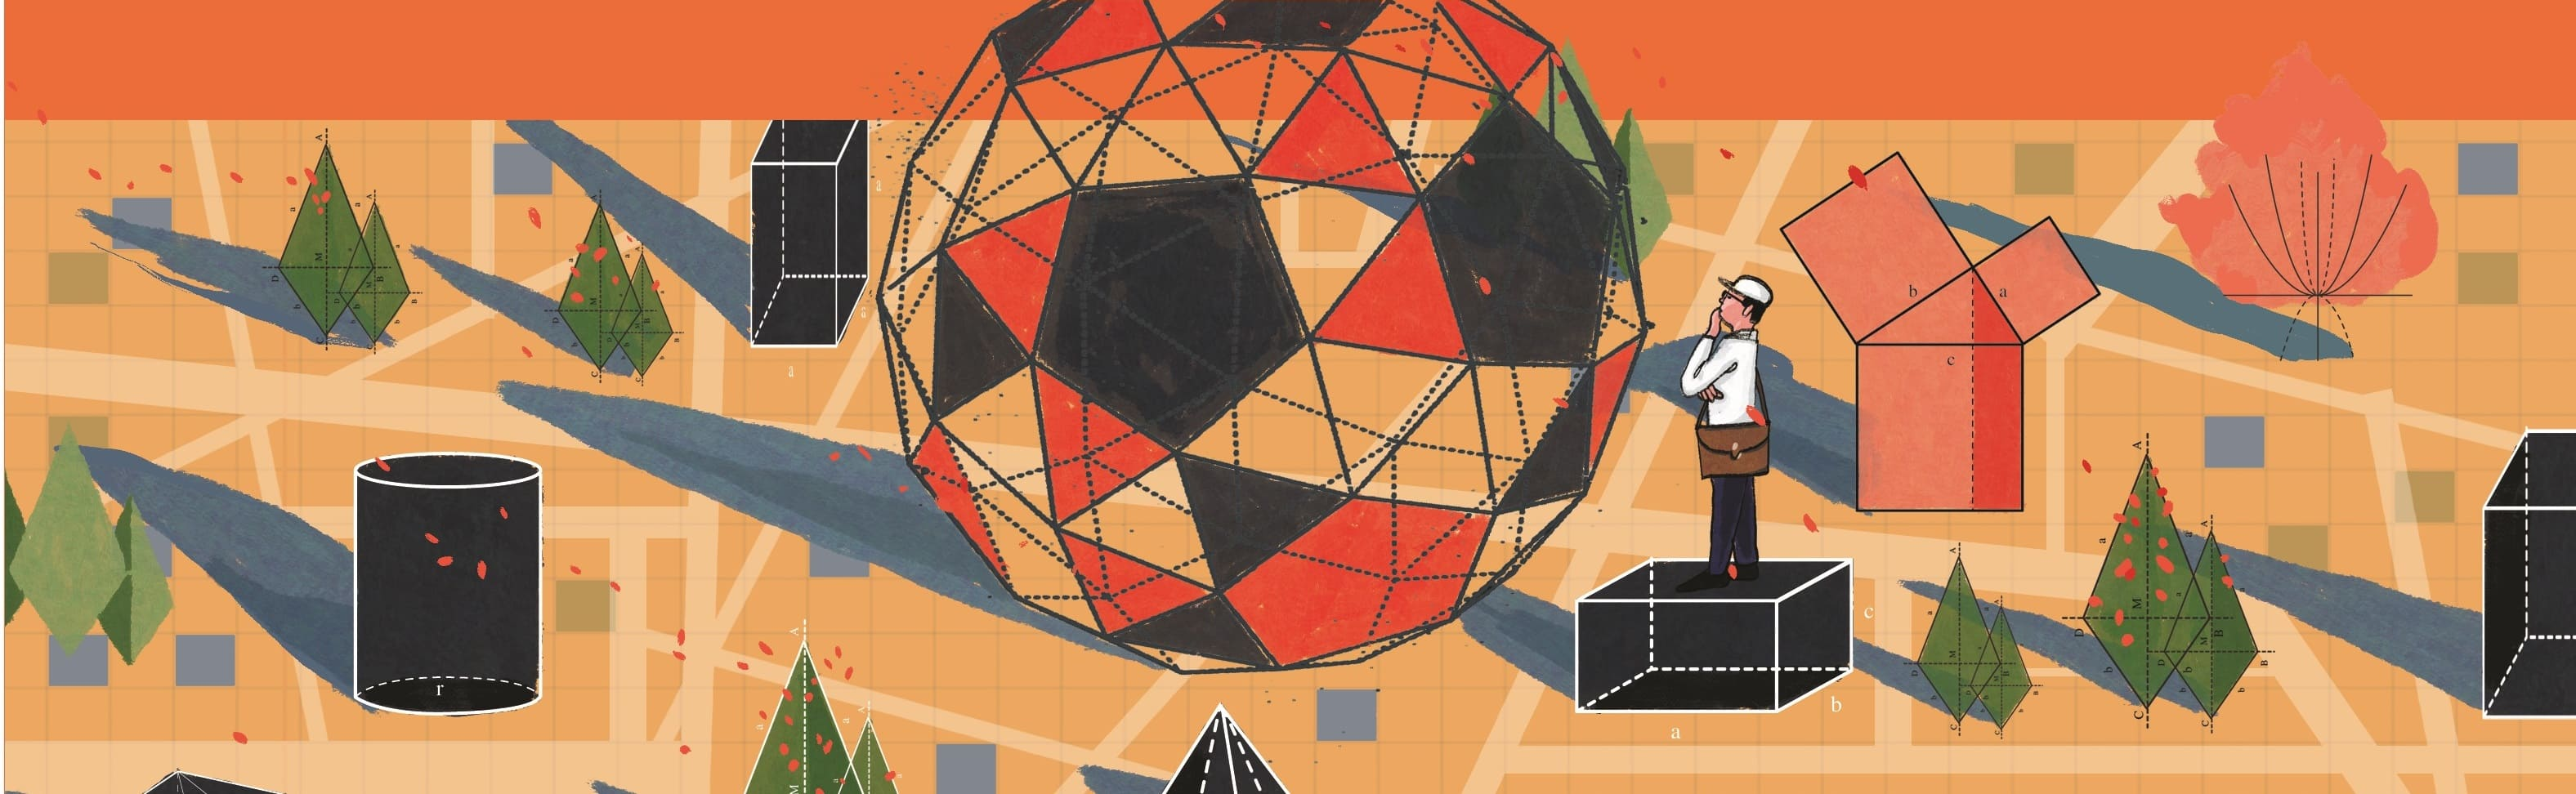
\includegraphics[width=19.3cm]{../bannerduongvao}}}
\AddToShipoutPicture*{\put(80,528){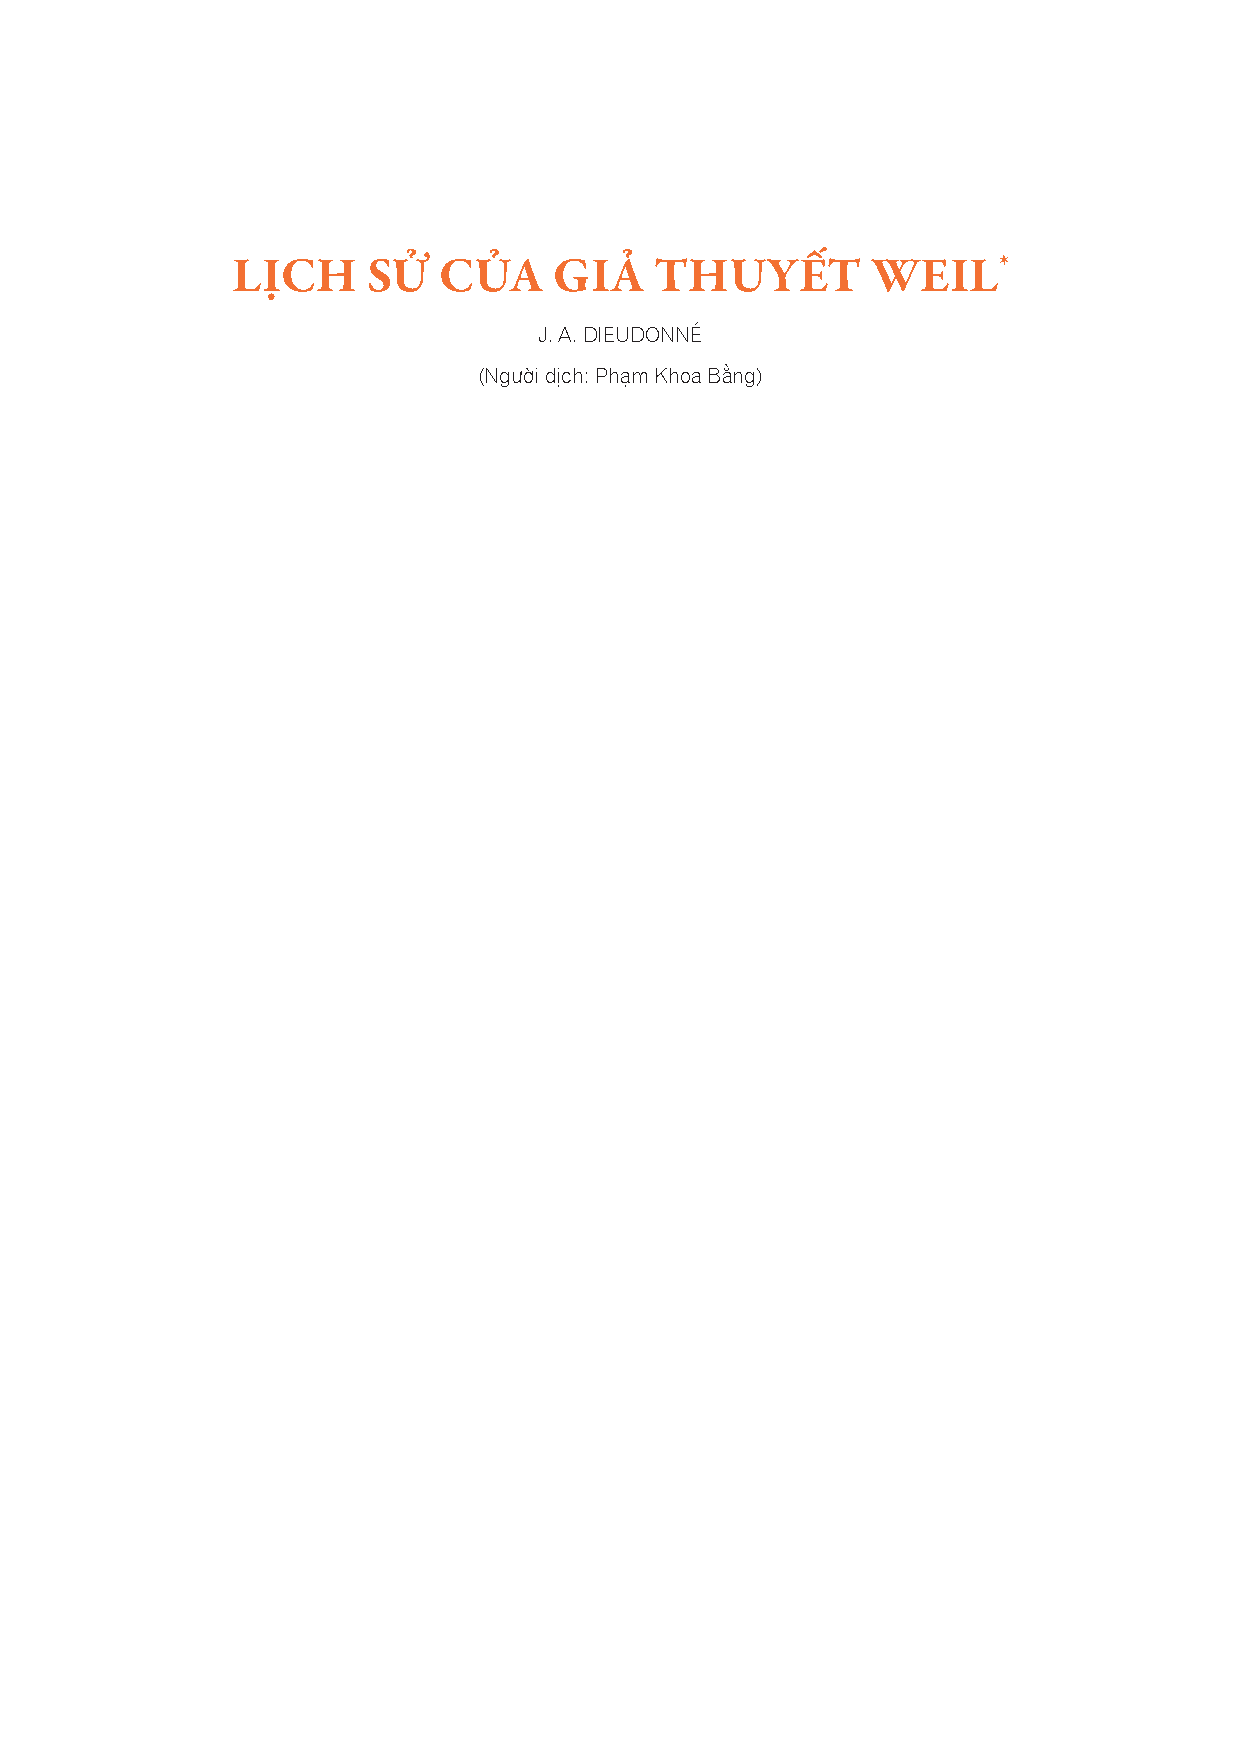
\includegraphics[scale=1]{../tieude.pdf}}}
\centering
\endgroup

\vspace*{180pt}

\begin{multicols}{2}	
	Câu chuyện của ``các giả thuyết Weil" là một ví dụ kỳ diệu của trí tưởng tượng toán học, và là một trong những thí dụ đáng ngạc nhiên nhất biểu lộ sự thống nhất cơ bản của toán học. Những ý tưởng cốt lõi dẫn tới chứng minh của chúng tới từ sáu người: E. Artin, F. K. Schmidt, H. Hasse, A. Weil, A. Grothendieck, và P. Deligne, trong khoảng năm mươi năm ($1923-1973$).
	\vskip 0.1cm
	$\pmb{1.}$ \textbf{\color{duongvaotoanhoc}Số nghiệm của phương trình đồng dư}
	\vskip 0.1cm
	Một cách đủ thích hợp, câu chuyện, như mọi vấn đề trong lý thuyết số, bắt đầu từ Gauss. Trong công trình về luật thuận nghịch bình phương của mình, ông đưa ra cái ngày nay được gọi là tổng Gauss (phổ biến nhất là tổng $\sum_{x=0}^{p-1} \mathrm{exp}(2\pi i x^2/p)$ với $p$ nguyên tố); để tính các tổng này, bằng một số lập luận sơ cấp, ông suy ra cần tính số nghiệm của các phương trình đồng dư có các dạng 
	\begin{align*}
			&ax^3 - by^3 \equiv 1 \ (\mathrm{mod} \ p),\\ 
			& ax^4 - by^4 \equiv 1 \ (\mathrm{mod} \ p), \tag{$1$}\\ 
			&y^2 \equiv ax^4 - 1 \ (\mathrm{mod} \ p)  
	\end{align*}
	trong đó $a,b$ là các số nguyên cố định không chia hết cho $p$, nghiệm $(x,y)$ được xét theo đồng dư modulo $p$ (như vậy các phương trình đồng dư $(1)$ được xem như các phương trình trong trường $\mathbb{F}_p$); và $p$ \textit{chạy} trong một tập vô hạn các số nguyên tố; chúng ta đi tìm những biểu diễn \textit{tiệm cận} (dưới dạng những hàm đơn giản của $p$) của số lượng các nghiệm. Một thời gian ngắn sau, Jacobi nhận xét rằng, ngược lại, bằng cách sử dụng các tính chất cơ bản của tổng Gauss, ta có thể thu được một đánh giá tốt về số nghiệm trong các trường hợp tổng quát hơn, ở đó các phương pháp sơ cấp trở nên cồng kềnh. Sau Jacobi, gần như không có nhiều tiến triển trong chủ đề này cho tới khi Hardy và Littlewood, trong khi nghiên cứu bài toán Waring để đưa ra các tính chất của ``chuỗi kỳ dị", thấy rằng cần phải đưa ra một đánh giá tiệm cận cho số nghiệm của phương trình đồng dư
	\begin{align*}
		x_1^k + ... + x_r^k \equiv 0 \ (\mathrm{mod} \ p), \tag{$2$}
	\end{align*}
	trong đó $p$ là một số nguyên tố chạy tới $+\infty$. Hai ông đã sử dụng phương pháp của Jacobi cho mục đích này; tổng quát hơn, năm $1949$, cả Hua-Vandier và A. Weil đã độc lập chứng minh rằng phương pháp này có thể đánh giá số nghiệm $N$ của những phương trình
	\begin{align*} 
		a_0x_0^{k_0} \!+\! ... \!+\! a_r x_r^{k_r} \!=\! 0 \ (a_0,...,a_r \neq 0)\tag{$3$}
	\end{align*}
	trong mọi \textit{trường hữu hạn} $\mathbb{F}_{q}$ với $q = p^m$ phần tử; kết quả được đưa ra
	\begin{align*}
		N = q^r + O(q^{(r+1)/2}). \tag{$4$}
	\end{align*}
	Kết quả tương tự được đưa ra bởi Davenport $(1931)$ và Mordell $(1933)$ cho các phương trình dạng $y^m = P_n(x)$ trên $\mathbb{F}_p$, trong đó $P_n$ là một đa thức bậc $n$; với một số giá trị $m,n$ nhỏ, họ thu được các đánh giá có dạng $N  = p + O(p^{\phi(m,n)})$ trong đó $1/2 < \phi(m,n) < 1$.
	\vskip 0.1cm
	$\pmb{2.}$ \textbf{\color{duongvaotoanhoc}Về hàm Zêta}
	\vskip 0.1cm
	Hãy để chúng tôi nhắc lại các tính chất cổ điển của hàm zêta Riemann: nó xác định với $\mathscr{R}(s) > 1$ bởi chuỗi $\zeta(s) = \sum_{n=1}^{\infty} n^{-s}$, và thỏa mãn phương trình Euler
	\begin{align*}
		\zeta(s) = \prod_p (1 - p^{-s})^{-1} \tag{$5$}
	\end{align*}
	trong đó tích chạy trên tập tất cả các số nguyên tố. Riemann chứng minh rằng $\zeta$ có thể thác triển thành một hàm phân hình trên mặt phẳng phức với một cực duy nhất tại $s=1$, và nếu đặt
	\begin{align*} 
		\xi = \frac{1}{2}s(s-1)\pi^{-s/2}\Gamma(s/2)\zeta(s),
	\end{align*}
	thì $\xi$ là một hàm chỉnh hình trên toàn bộ mặt phẳng phức và thỏa mãn phương trình hàm $\xi(s) = \xi(1-s)$. Hơn nữa ông đề xuất \textit{giả thuyết Riemann} (vẫn chưa được chứng minh) rằng mọi nghiệm của $\xi$ nằm trên đường thẳng $\mathscr{R}(s)=1/2$. 
	\vskip 0.1cm
	Một thời gian ngắn sau, Dedekind mở rộng lý thuyết của Riemann lên một trường số $K$ (mở rộng hữu hạn của $\mathbb{Q}$), bằng cách định nghĩa $\zeta_K(s) = \sum_{\mathfrak{a}}(N\mathfrak{a})^{-s}$, trong đó $\mathfrak{a}$ chạy trên tất cả các ideal của vành $\mathfrak{o}$ các số đại số nguyên trong $K$, \textit{chuẩn} $N\mathfrak{a}$ là số phần tử của vành $\mathfrak{o}/\mathfrak{a}$. Ông mở rộng công thức Euler thành
	\begin{align*}
		\zeta_K(s) = \prod_{\mathfrak{p}} (1-  (N\mathfrak{p})^{-s})^{-1}, \tag{$6$}
	\end{align*}
	trong đó tích chạy trên tất cả các ideal nguyên tố $\mathfrak{p}$ của $\mathfrak{o}$; rất nhiều năm sau Hecke chứng minh rằng $\zeta_K$ có thể thác triển thành một hàm phân hình và thỏa mãn một phương trình hàm tương tự như phương trình hàm Riemann cho $\xi$. 
	\vskip 0.1cm
	Một cách hình thức, ta thấy rằng phương trình ($6$) chỉ dùng hai tính chất của vành $\mathfrak{o}$: $1)$ $\mathfrak{o}$ là một vành Dedekind: $2)$ trường $\mathfrak{o}/\mathfrak{p}$ là hữu hạn với mọi ideal nguyên tố $\mathfrak{p}$: thật vậy, nếu $\mathfrak{a} = \mathfrak{p}_1^{v_1}...\mathfrak{p}_r^{v_r}$ là một phân tích thành các ideal nguyên tố của ideal $\mathfrak{a}$ thì $\mathfrak{o}/\mathfrak{a}$ đẳng cấu với tích trực tiếp của các $\mathfrak{o}/\mathfrak{p}_i^{v_i}$, và với mọi ideal nguyên tố $\mathfrak{p}$, mỗi $(\mathfrak{o}/\mathfrak{p})$--module $\mathfrak{p}^h/\mathfrak{p}^{h+1}$ đẳng cấu với $\mathfrak{o}/\mathfrak{p}$; điều đó chứng tỏ rằng chuẩn là nhân tính, từ đó suy ra ($6$) một cách hình thức (chứng minh tính hội tụ của tích vô hạn cần một số ước lượng đơn giản về số các ideal nguyên tố với chuẩn cho trước). Năm $1923$, E. Artin nhận xét rằng các tính chất này đúng cho các vành định nghĩa theo cách sau: bắt đầu với một trường hữu hạn $\mathbb{F}_q$, xét trường $K_0 = \mathbb{F}_q(T)$ các phân thức hữu tỷ, và một mở rộng toàn phương $K = K_0(v)$ với $v^2=P(T)$, trong đó $P$ là một đa thức không có nghiệm bội. Khi đó bao đóng nguyên $\mathfrak{o}$ của $\mathbb{F}_q[T]$ trong $K$ thỏa mãn các tính chất $1)$ và $2)$, $\mathfrak{o}/\mathfrak{p}$ là một \textit{mở rộng hữu hạn} của $\mathbb{F}_q$ với mỗi ideal nguyên tố $\mathfrak{p}$; rất dễ để chứng minh chuỗi và tích vô hạn trong định nghĩa của $\zeta_K$ hội tụ với $\mathscr{R}(s)>1$. Hơn nữa Artin còn thấy rằng lý thuyết này đơn giản hơn của Dedekind rất nhiều, lý do là các hàm của ông có thể viết dưới dạng $Z(q^{-s})$ trong đó $Z(u)$ là một \textit{hàm hữu tỷ} với hệ số trong $\mathbb{Q}$; phương trình hàm biểu diễn thương $Z(1/qu)/Z(u)$ bởi một hàm hữu tỷ với không điểm và cực cho trước; ông ấy sau đó giả thuyết rằng không điểm của $Z(u)$ tất cả đều nằm trên đường tròn $\left| u \right| = q^{1/2}$ và tự kiểm chứng giả thuyết này với rất nhiều đa thức $P$ bậc nhỏ. 
	\vskip 0.1cm
	Bây giờ các ideal nguyên tố $\mathfrak{p}$ sao cho $\mathfrak{o}/\mathfrak{p} \cong \mathbb{F}_q$ ($N\mathfrak{p}=q$) tương ứng một-một với các đồng cấu $\mathfrak{o} \to \mathbb{F}_q$; mọi đồng cấu như vậy gửi $(T,v)$ tới $(a,b) \in \mathbb{F}_q^2$ thỏa mãn $b^2=P(a)$. Nói cách khác số nghiệm của phương trình $y^2 = P(x)$ trong $\mathbb{F}_q^2$ chính là số lượng $N_1$ các ideal nguyên tố kiểu này; tuy nhiên từ phương trình Euler ($6$) suy ra luôn rằng 
	\begin{align*} 
		\log Z(u) = N_1 u + \cdots 
	\end{align*}
	gần $u=0$, như vậy nghiên cứu $Z(u)$ giúp ta hiểu về $N_1$. ``Giả thuyết Riemann" của Artin sinh ra đánh giá
	\begin{align*}  
		\left|N_1 -q \right| \leq  c \cdot q^{1/2}, \tag{$7$}
	\end{align*}
	và như vậy làm chặt hơn những kết quả trước đó của ông về bài toán đồng dư của Gauss. 
	\vskip 0.1cm
	$\pmb{3.}$ \textbf{\color{duongvaotoanhoc}Bước vào hình học đại số}
	\vskip 0.1cm
	Cho $k$ là một trường giao hoán bất kỳ, người ta cố gắng hình dung tập nghiệm $(x_1,...,x_r) \in k^r$ của một phương trình $P(x_1,...,x_r)=0$, với $P$ là một đa thức bất khả quy trong $k[T_1,...,T_r]$ xem như một ``siêu mặt đại số affine" (``đường cong" với $r=2$, ``mặt" với $r=3$) trong ``không gian affine" $k^r$, Hơn nữa, với mọi mở rộng trường $K \supset k$, ta có thể xét các nghiệm của $P(y_1,...,y_r)$ với giá trị $y_i$ trong trường $K$ \textit{lớn hơn}, như vậy ta có một ``siêu mặt đại số" $V$ trong ``không gian affine" $K^r$; việc các hệ số của $P$ nằm trong $k$ giờ được thay bởi việc nói $V$ \textit{xác định} trên $k$. Kinh nghiệm cho thấy việc chuyển đổi giữa ngôn ngữ hình học và trực giác sang những đa tạp ``trừu tượng"chỉ có ích khi $K$ là \textit{đóng đại số} (hãy thử nghĩ về $x_1^2+x_2^2+1=0$ khi $k=\mathbb{R}$). Ta sẽ hạn chế sự quan tâm xuống trường hợp $K=\overline{k}$, bao đóng đại số của $k$; hơn nữa, ta chỉ xét các siêu mặt $V$ không kỳ dị trong $\overline{k}^r$, i.e. tại các điểm mà ``siêu phẳng tiếp xúc" được định nghĩa duy nhất theo nghĩa thông thường (có nghĩa là tất cả các đạo hàm riêng không đồng thời triệt tiêu trong $V$). Với mọi điểm $x=(x_1,...,x_r) \in V$, toạ độ $x_i$ nằm trong $\overline{k}$, do đó có một mở rộng hữu hạn nhỏ nhất $k(x)$ của $k$ chứa tất cả $x_j$ và $[k(x):k]=\mathrm{deg}(x)$ được gọi là \textit{bậc} của điểm $x$. Nếu $\mathfrak{m}$ là hạt nhân của đồng cấu $k[T_1,...,T_r] \to \overline{k}$ gửi mỗi $T_i$ tới $x_i$ thì $\mathfrak{m}$ là một ideal cực đại của $k[T_1,....,T_r]$ và $k[T_1,...,T_r]/\mathfrak{m}$ đẳng cấu với $k(x)$; ta viết $k(\mathfrak{m})=k(x)$ và $\mathrm{deg}(\mathfrak{m}) =\mathrm{deg}(x)$; có thể chứng minh rằng mọi ideal cực đại $\mathfrak{m}$ của $k[T_1,...,T_r]$ chứa $P(T_1,...,T_r)$ ứng với một điểm $x$ của $V$ với bậc $\mathrm{deg}(\mathfrak{m})$. 
	\vskip 0.1cm
	Khi $k=\mathbb{F}_q$, đặt
	\begin{align*}
		Z_V(u) = \prod_{P \in \mathfrak{m}}(1 - u^{\mathrm{deg}(\mathfrak{m})})^{-1}; \tag{$8$}
	\end{align*}
	hàm $Z(u)$ định nghĩa bởi E. Artin bằng với hàm $Z_C(u)$, trong đó $C$ là ``đường cong affine" $x_2^2 - P(x_1) = 0$ xác định trên $\mathbb{F}_q$. Một cách tổng quát ta gọi $Z_V$ là \textit{hàm zêta} của $V$. Các điểm của $V$ trong $(\mathbb{F}_q)^r$ là các điểm mà $\mathrm{deg}(x)$ là ước của $n$; hiển nhiên số lượng các điểm như vậy $\leq q^{nr}$, như vậy số lượng các ideal cực đại $\mathfrak{m}$ mà $P \in \mathfrak{m}$, tương ứng với các điểm này, có ước lượng \textit{tiên nghiệm} $\leq q^{nr}$, điều này chứng tỏ rằng ($8$) hội tụ với $u$ nhỏ; hơn nữa, với $u$ nhỏ ta có thể viết
	\begin{align*}
			uZ'_V(u)/Z_V(u) & = \sum_{P \in \mathfrak{m}} \frac{\mathrm{deg}(\mathfrak{m}) u^{\mathrm{deg}(\mathfrak{m})}}{1 - u^{\mathrm{deg}(\mathfrak{m})}} \\ 
			& = \sum_{v=1}^{\infty} \sum_{P \in \mathfrak{m}} \mathrm{deg}(\mathfrak{m}) u^{v\mathrm{deg}(\mathfrak{m})} \\
			&= \sum_{v=1}^{\infty} N_v u^v\tag{$9$}
	\end{align*}
	trong đó $N_v$ là số điểm của $V$ trong $(\mathbb{F}_{q^v})^r$.  
	\vskip 0.1cm
	Cách định nghĩa này có thể mở rộng cho các dạng đa tạp không kỳ dị khác, không nhất thiết phải bị nhúng trong ``không gian affine" $\overline{k}^r$. Nói một cách theo lịch sử, ngôn ngữ của hình học đại số trong lý thuyết của các hàm zêta được giới thiệu vào năm $1931$ bởi F. K. Schmidt, người nghiên cứu các \textit{đường cong xạ ảnh} không kỳ dị trên trường hữu hạn $\mathbb{F}_q$. Ông chứng minh rằng lý thuyết Dedekind--Weber của đường cong đại số trên $\mathbb{C}$ (bao gồm định nghĩa về giống và định lý Riemann--Roch) có thể mở rộng cho đường cong xạ ảnh trên một trường đóng đại số $\overline{k}$ bất kỳ; điều này cho phép ông chứng minh rằng với mọi đường cong xạ ảnh không kỳ dị $C$ với giống $g$ định nghĩa trên $\mathbb{F}_q$, hàm zêta có thể biểu diễn dưới dạng
	\begin{align*} 
		Z_C(u) = P_{2g}(u)/(1-u)(1-qu) \tag{$10$}
	\end{align*}
	trong đó tử số là một đa thức bậc $2g$ với hệ số nguyên và ta có một phương trình hàm
	\begin{align*} 
		Z_C(1/qu) = (qu^2)^{1-g}Z_C(u). \tag{$11$}
	\end{align*}
	``Giả thuyết Riemann" cho $C$ do đó nói rằng các không điểm của $P_{2g}$ nằm trên đường tròn $\left|u \right|=q^{1/2}$; dễ thấy điều này tương đương với bất đẳng thức
	\begin{align*} 
		\left|N_v \!-\! q^v\!-\! 1\right| \!\leq\! 2g \!\cdot\! q^{1/2} \ \text{với mọi} \ v \geq 1. \tag{$12$}
	\end{align*}
	$\pmb{4.}$ \textbf{\color{duongvaotoanhoc}Mơ mộng về Tôpô đại số}
	\vskip 0.1cm
	Quay lại trường hợp siêu mặt $V$ trong $(\overline{\mathbb{F}}_q)^r$, nhận xét rằng các phần tử của $\overline{\mathbb{F}}_q$ thuộc $\mathbb{F}_{q^n}$ chính là những phần tử mà $t^{q^n}=t$. Xét ánh xạ
	\begin{align*}
		\Phi: (x_1,...,x_r) \mapsto (x_1^{q},...,x_r^q)
	\end{align*}
	từ $(\overline{\mathbb{F}}_q)^r$ vào chính nó. Do hệ số của $P$ nằm trong $\mathbb{F}_q$, do đó thỏa mãn $t^q = t$, ta có
	\begin{align*}
		P(\Phi(x)) = (P(x))^q,
	\end{align*}
	do đó $\Phi$ ánh xạ $V$ lên chính nó; hạn chế của $\Phi$ lên $V$ được gọi là cấu xạ Frobenius của $V$. Năm $1936$, Hasse nhận thấy rằng với một đường cong $C$, số $N_v$ chính là số điểm $x \in C$ thỏa mãn $\Phi^v(x) = x$; i.e. $x$ là một \textit{điểm bất động} của $\Phi^v$. Bây giờ, chúng ta hãy bỏ qua chuỗi các sự kiện mang tính niên đại mà giả vờ rằng ta đang làm việc với các đa tạp đại số không kỳ dị ``cổ điển" $X$ trong một không gian xạ ảnh phức. Từ thời của Picard và  Poincaré người ta đã nhận thấy rằng hầu hết các tính chất của các đa tạp đại số được liên hệ chặt chẽ với các tính chất \textit{đồng điều}. Trong phiên bản hiện thời (chủ yếu từ các công trình của Lefschetz và Hodge), với một đa tạp xạ ảnh không kỳ dị bất khả quy $X$ chiều $d$ trên $\mathbb{C}$ (do đó là một đa tạp khả vi chiều $2d$), các tính chất này xoay quanh \textit{đại số đối đồng điều} $H^{\bullet}(X) = \bigoplus_i H^i(X)$ của $X$ trên trường $K$ với \textit{đặc số} $0$; nó là một đại số phân bậc trên $K$, thỏa mãn các tính chất sau:
	\vskip 0.1cm
	($A$) $1.$ Mỗi $H^i(X)$ là một $K$--không gian vector hữu hạn chiều, bằng $0$ ngoại trừ $0 \leq i \leq 2d$;
	\vskip 0.1cm
	$2.$ Tồn tại một đẳng cấu tự nhiên $H^{2d}(X) \overset{\sim}{\longrightarrow} K$, và với mỗi $i$, phép nhân trên $H^{\bullet}(X)$ cho ta một phép ghép cặp không kỳ dị $H^{i}(X) \times H^{2d-i}(X) \to H^{2d}(X) \overset{\sim}{\longrightarrow} K$ (đối ngẫu Poincaré) cho phép ta đồng nhất $H^{2d-i}(X)$ với 
	\begin{align*} 
		H_i(X) = \mathrm{Hom}_K(H^i(X),K),
	\end{align*} 
	\textit{đồng điều} của $K$ tại chiều $i$.
	\vskip 0.1cm
	$3.$ Với các đa tạp không kỳ dị $X, Y$, tồn tại một đẳng cấu tự nhiên của các đại số phân bậc 
	\begin{align*} 
		&H^{\bullet}(X) \otimes H^{\bullet}(Y) \cong H^{\bullet}(X \times Y) \\
		&\text{(công thức Kunneth)}.
	\end{align*}
	($B$) Mọi cấu xạ $f: X \to X$ định nghĩa tự nhiên, với mỗi $i$, một đồng cấu tuyến tính $f^{(i)}:H^i(X) \to H^i(X)$, sao cho các $f^{(i)}$ với $0 \leq i \leq 2d$ cảm sinh một đồng cấu $f^{\bullet}:H^{\bullet}(X) \to H^{\bullet}(X)$ của các đại số phân bậc. Các \textit{điểm bất động} của $f$ là phép chiếu lên $X$ của giao của đồ thị $\Gamma$ của $f$ và đường chéo $\Delta$ của $X \times X$; nếu $\Gamma$ giao \textit{hoành} với $\Delta$ tại mỗi điểm (nghĩa là các không gian tiếp xúc của chúng có giao chỉ là một điểm), số lượng điểm bất động của $f$ được tính bởi \textit{công thức vết Lefschetz}
		\begin{align*} \label{eq:13}
			N  = \sum_{i=0}^{2d} (-1)^i \mathrm{Tr}(f^{(i)}). \tag{$13$}
		\end{align*}
	($C$) Nếu $Y$ là một đa tạp con không kỳ dị của $X$ với chiều $d-1$, các ánh xạ tuyến tính tự nhiên $H^i(X) \to H^i(Y)$ là song ánh với $i \leq d-2$ và đơn ánh với $i = d-1$. 
	\vskip 0.1cm
	($D$) Lấy $h \in H^2(X)$ từ đối ngẫu Poincaré ứng với lớp đồng điều trong $H_{2d-2}(X)$ của một lát cắt siêu phẳng của $X$, và xét $L: a \to ha$ là phép nhân trái bởi $h$ trong $H^{\bullet}(X)$; khi đó $L^{d-i}: H^i(X) \to H^{2d-i}(X)$ là một đẳng cấu với $i \leq d$.
	\vskip 0.1cm
	Một lập luận đại số đơn giản cho thấy nếu một cấu xạ $f: X \to X$ thỏa mãn $f^{(2)}(h) = q \cdot h$ với $q > 0$ là một số hữu tỷ, và nếu $g_i = q^{-i/2}f^{(i)}$ (xem như một tự đồng cấu của $H^{i}(X) \otimes_K \overline{K}$), $g_i$ là song ánh, và $g_i^{-1}$ được đồng nhất với $\text{}^tg_{2d-i}$ bởi đối ngẫu Poincaré. Điều này suy ra rằng nếu $\alpha_{ij}$ là các giá trị riêng của $f^{(i)}$ trong $\overline{K}$, tập các phần tử $q^{i/2}\alpha_{ij}$ trùng với tập các phần tử $\alpha_{2d-i,j}/q^{d-(i/2)}$.
	\vskip 0.1cm
	($E$) Trong mỗi $H^i(X)$ với $i \leq d$ có một không gian con $A^i(X)$ ổn định dưới tác động của $f^{(i)}$ với mọi cấu xạ $f: X \to X$, và trên mỗi $A^i(X)$, ta có thể trang bị một cấu trúc không gian vector trên trường các số hữu tỷ cùng một \textit{tích vô hướng} không kỳ dị, sao cho: với mỗi $f$ thỏa mãn ($D$) thì mỗi $g_i$ là ánh xạ \textit{unita} với tích vô hướng này; điều này suy ra tất cả các giá trị riêng của $f^{(i)}$ (là các phần tử của $\overline{\mathbb{Q}}$) có giá trị tuyệt đối là $q^{1/2}$.
	\vskip 0.1cm
	Quay lại với siêu mặt $V$ xác định trên $\mathbb{F}_q$, \textit{giả sử} ta có thể gán với nó một đại số phân bậc $H^{\bullet}(V)$ có tất cả các tính chất vừa nêu, hơn nữa $\Phi^{(2)}(h) = q \cdot h$ trong đó $\Phi$ là đồng cấu Frobenius. Dễ thấy đồ thị của $\Phi^v$ giao hoành với $\Delta$; do đó, nếu $\alpha_{ij}$ là các giá trị riêng của $(\Phi^v)^{(i)}$, số $N_v$ có thể cho bởi công thức
	\begin{align*} 
		N_v = \sum_i (-1)^i \sum_j \alpha_{ij}^v;\tag{$14$}
	\end{align*}
	và do đó ta có (với $d= r-1=\mathrm{dim}(V)$)
	\begin{align*} \label{eq:15}
		Z_V(u) = \frac{P_1(u)P_3(u)...P_{2d-1}(u)}{P_0(u)P_2(u)...P_{2d}(u)} \tag{$15$}
	\end{align*}
	trong đó $P_i(u) = \mathrm{deg}(1 - u \cdot \Phi^{(i)})$ là một đa thức với hệ số nguyên. Nói riêng, $Z_V(u)$ là một hàm \textit{hữu tỷ}; hơn nữa $Z_V(1/q^d u)$ nên có không điểm và cực giống với $Z_V(u)$ ngoại trừ khi $u=0$, và ta nên có $\left|\alpha_{ij}\right|=q^{1/2}$. Cuối cùng, nếu tất cả hệ số của $V$ là các lớp đồng dư mod $p$ của các số nguyên, hệ số của một phương trình của một đa tạp không kỳ dị $V_0$ trong $\overline{\mathbb{Q}}^r$, bậc của mỗi $P_i$ sẽ bằng số Betti thứ $i$ của $V_0$. 
	\vskip 0.1cm
	Các phát biểu trên là \textit{các giả thuyết Weil} cho $Z_V$.
	\vskip 0.1cm
	$\pmb{5.}$ \textbf{\color{duongvaotoanhoc}Những ``phương án thay thế" cho đối đồng điều của Hasse và Weil} 
	\vskip 0.1cm
	Để hiểu tại sao Weil đã có thể đi tới những khái niệm táo bạo như vậy, ta phải quay lại những ý tưởng đầu tiên của Hasse trong việc chứng minh ``giả thuyết Riemann" cho các đường cong \textit{giống} $1$ trên $\mathbb{F}_q$. Trong lý thuyết cổ điển của các đường cong không kỳ dị trên trường số phức, mỗi đường cong $C$ được gán với \textit{jacobian} $J = J(C)$, có thể xem như đối ngẫu Pontrjagin của nhóm đồng điều $H_1(C,\mathbb{Z})$; đối ngẫu này được dẫn ra từ dạng song tuyến tính $(\gamma,\omega) \mapsto \int_{\gamma}\omega$ định nghĩa trên các chu trình $\gamma$ và các dạng vi phân abel chỉnh hình $\omega$ trên diện Riemann $C$ (``chu kỳ" của $\omega$ trên $\gamma$). Nếu $C$ có giống $g$ thì $J(C)$ là một xuyến phức $\mathbb{C}^g/\Delta$ trong đó $\Delta$ là một nhóm con rời rạc với hạng $2g$, thỏa mãn các điều kiện song tuyến tính Riemann cổ điển. Ta có thể định nghĩa $J$ một cách đại số, bằng cách xét các nhóm cộng $G/G_i$ của các lớp của các ước bậc $0$ trên $C$, modulo quan hệ tương đương tuyến tính: ta gắn mỗi ước $D$ bậc $0$, vốn có thể viết dưới dạng $\partial \gamma$ với $1$-xích $\gamma$ trên diện Riemann, một lớp $\phi(D)$ trong $\mathbb{C}^g/\Delta$ của vector $\left(\int_{\gamma}\omega_1,...\int_{\gamma}\omega_g\right)$, trong đó các $\omega_j$ lập thành một cơ sở của không gian các dạng vi phân chỉnh hình; định lý Abel-Jacobi nói rằng phép tương ứng này là toàn ánh và có hạt nhân $G_i$. Từ đó có thể trang bị cho $J$ một cấu trúc \textit{nhóm đại số} (một trường hợp cụ thể của nhóm đại số trên $\mathbb{C}$ được biết đến như \textit{các đa tạp abel}) với sự giúp đỡ của các điều kiện (siêu việt) song tuyến tính Riemann. Cuối cùng, nếu $x_0$ là một điểm trên $C$,
	\begin{align*}
		x \mapsto \phi((x) - (x_0))
	\end{align*}
	là một cấu xạ từ $C$ vào $J$ và là đẳng cấu nếu $g=1$.
	\vskip 0.1cm
	Phương pháp đầu tiên của Hasse để làm việc với các đường cong $C$ giống $1$ xác định trên $\mathbb{F}_q$ là ``nâng" $C$ thành một đường cong $C_0$ ``cổ điển" giống $1$ xác định trên trường các số hữu tỷ $\mathbb{Q}$: nếu $E$ là trường các hàm hữu tỷ trên $C$, ông chứng minh rằng ta có thể xác định $C_0$ sao cho, nếu $\omega_1,\omega_2$ là các hàm chu kỳ của các hàm elliptic ứng với $C_0$ (nên trường $E_0$ của các hàm này là trường các hàm hữu tỷ trên $C_0$), $\omega_1/\omega_2$ phải sinh ra một trường toàn phương ảo $K$ trên $\mathbb{Q}$, và $E$ sẽ là trường thặng dư của vành các số nguyên của $K$ modulo một ideal nguyên tố khéo chọn nào đó. Hasse từ đó đã có thể dùng các kết quả cổ điển về ``các phép nhân phức" của $C_0$ (i.e. tự đồng cấu của jacobian $J(C_0)$) để xác định số điểm của $C$ với bậc $1$, và chứng minh ``giả thuyết Riemann" cho $C$.
	\vskip 0.1cm
	Một thời gian ngắn sau, Hasse từ bỏ phương pháp trên và thay thế bằng một phương pháp có tính nội tại hơn: như đã nói ở trên, $J(C)$ có thể định nghĩa một cách đại số như một nhóm ``trừu tượng", và cấu xạ Frobenius định nghĩa tự nhiên một tự đồng cấu của nhóm đó; Hasse chứng minh rằng tử số của hàm zêta $Z_C$ trong ($10$) (trong trường hợp này là một đa thức bậc $2$) được đồng nhất với đa thức đặc trưng của tự đồng cấu đó. Công cụ mà ông giới thiệu cho mục đích này là một số nguyên $v(\lambda)$ gắn với mỗi tự toàn cấu $\lambda$ của $J(C)$: nếu $E$ là trường các hàm hữu tỷ của $C$, $\lambda$ định nghĩa một ``đối cấu xạ" (comorphism) $R(\lambda)$, một tự đẳng cấu của $E$ và $v(\lambda)$ là bậc $[E:R(\lambda)(E)]$, hữu hạn khi $\lambda$ là toàn cấu. Hasse chứng minh rằng với mọi số nguyên $a,b$ thì
	\begin{align*} v(a.1 + b.\lambda) = a^2 + \sigma(\lambda)ab + v(\lambda)b^2
	\end{align*} 
	với mọi tự toàn cấu $\lambda$ của $J(C)$, tính xác định dương của dạng toàn phương này cho ông chứng minh của ``giả thuyết Riemann". 
	\vskip 0.1cm
	Việc mở rộng những ý tưởng này cho các đường cong $C$ giống $g$ bất kỳ trên $\mathbb{F}_q$ là không hề hiển nhiên: lý thuyết cổ điển chứng minh rằng $J(C)$ nên là một nhóm đại số $g$ chiều (thay vì đẳng cấu với $C$ như một đa tạp đại số trong trường hợp của Hasse), và cho tới tận năm $1940$ không ai mở rộng lý thuyết của các nhóm đại số trên trường đặc số $p>0$ sang hình học đại số, và nói riêng lý thuyết của các đa tạp abel. Điều này đã được thực hiện một mình bởi A. Weil, người đầu tiên phải phát triển, trong cuốn sách nổi tiếng \textit{Foundations of algebraic geometry}, các tính chất cơ bản của các số giao một cách độc lập mà không viện tới tôpô đại số. Sau đó ông đã có thể nghiên cứu cấu trúc vành của các tự đồng cấu của một đa tạp abel $A$; với mọi tự toàn cấu $\lambda$ của $A$, Weil định nghĩa số nguyên $v(\lambda)$ như Hasse, (bây giờ $E$ là trường các hàm hữu tỷ trên $A$) và lần này chứng minh
	\begin{align*}
		&v(a \cdot 1 + b \cdot \lambda) \\
		= \,&a^{2g} + \sigma(\lambda)a^{2g-1}b +...+ v(\lambda)b^{2g}.
	\end{align*}
	Bất biến $\sigma(\lambda)$ được xem như một ``thay thế" đóng vai trò của $\mathrm{Tr}(f^{(1)})$ khi $\lambda$ là tự đồng cấu của $J(C)$ ứng với một cấu xạ $f$ của $C$. Một ``thay thế" cho đối ngẫu Poincaré được phát hiện trong một đối ngẫu tổng quát cho các đa tạp abel mà có thể định nghĩa nghĩa hoàn toàn đại số (trong trường hợp cổ điển người ta định nghĩa nó bởi đối ngẫu Pontrjagin); cuối cùng, nếu $\lambda'$ là ``chuyển vị" của một tự đồng cấu $\lambda$ trong đối ngẫu này thì ta có thể chứng minh $\sigma(\lambda \lambda') > 0$ với $\lambda \neq 0$, tính chất này (xem như một ``thay thế" cho tính xác định dương của tích vô hướng Hodge) cho phép Weil đưa ra chứng minh của ``giả thuyết Riemann" cho đường cong có giống bất kỳ.
	\vskip 0.1cm
	Trong tất cả các công trình này, Weil đã không ngừng giữ trong trí óc ông lý thuyết cổ điển của các ``tương ứng" phát triển bởi Hurwicz: một tương ứng trên $C$ có thể xem như một cấu xạ ``đa trị", mà cụ thể hơn như một đường cong $\Gamma$ trên diện $C \times C$; tốt hơn nữa, nó được định nghĩa như một ước (tổ hợp tuyến tính của các đường cong) trên $C \times C$. Một tương ứng $\Gamma$ gắn một cách tự nhiên (bắt chước phiên bản lý thuyết tập hợp) mỗi ước $D$ trên $C$ (tổ hợp tuyến tính của các điểm) một ước khác $\Gamma(D)$, một lần nữa điều này định nghĩa một tự đồng cấu của $J(C)$; ngược lại có thể chỉ ra rằng mọi tự đồng cấu của $J(C)$ đều thu được từ cách định nghĩa này. Trong trường hợp cổ điển, công thức Lefschetz ($13$) có thể được mở rộng để cho số giao của một tương ứng $\Gamma$ với ``tương ứng đồng nhất", i.e. đường chéo $\Delta$ của $C \times C$, và thực tế điều này đã được chứng minh bởi Hurwicz vào năm $1866$, sử dụng lý thuyết tích phân abel; sự thật là Weil đã có thể chứng minh một công thức tương tự bằng các công cụ thuần túy đại số, điều đã dẫn ông đến chỗ đề xuất các giả thuyết mang tên mình.
	\vskip 0.1cm
	$\pmb{6.}$ \textbf{\color{duongvaotoanhoc}Đối đồng điều \'etale và định lý của Deligne}
	\vskip 0.1cm
	Sử dụng kết quả của mình cho các đường cong, Weil đã chứng minh được các giả thuyết của chính ông với các siêu mặt dạng ($3$), cũng như cho những đa tạp khác như các đa tạp Grassman. Nhưng tại thời điểm đó không có một lý thuyết đối đồng điều nào đủ ``tốt" đã được định nghĩa. Khoảng năm $1953$, Cartan và Serre đã dùng đối đồng điều Leray với hệ số là các bó như một công cụ cực kỳ hữu hiệu để nghiên cứu các đa tạp phức, và Serre đã chỉ ra làm cách nào để chuyển các kỹ thuật này sang các đa tạp đại số trên một trường đóng đại số với đặc số $p$. Nhưng khi $p>0$, những nhóm đối đồng điều mới đó được định nghĩa hiển nhiên không thể được sử dụng bởi công thức Lefschetz ($13$), trong đó vế trái bắt buộc phải là một số nguyên, mà không phải một phần tử của một trường có đặc số $p$. Chỉ sau khi Grothendieck xây dựng lý thuyết lược đồ mà, từ một lưu ý của Serre, thì cậu ấy đã có thể mở rộng ý tưởng ban đầu theo cả hai hướng ``tôpô" và ``bó", gắn mỗi đa tạp (hoặc lược đồ) $X$ một đại số đối đồng điều $H^{\bullet}(X_{et},\mathbb{Q}_l)$ trên trường $l$--adic $\mathbb{Q}_l$, trong đó $l$ là một số nguyên tố khác với đặc số của trường ban đầu (sự can thiệp của các trường $l$--adic trong những câu hỏi này đã được nhận ra bởi Weil và Deuring).
	\vskip 0.1cm
	Độ sâu sắc và phức tạp của các kỹ thuật liên quan trong định nghĩa của ``đối đồng điều \'etale" $H^{\bullet}(X_{et})$ như thể để loại trừ mọi khả năng trong việc đưa ra bất kỳ một chi tiết nào nữa trong định nghĩa của nó. Hãy để chúng tôi chỉ ra Grothendieck (với sự giúp đỡ của M. Artin (con trai của E. Artin) và J. L. Verdier) đã có thể chứng minh các tính chất ($A$), ($B$), ($C$) \footnote[1]{\color{duongvaotoanhoc}Trước khi đối đồng điều $l$--adic được định nghĩa, Dwork đã chứng minh, bằng cách khéo léo sử dụng các hàm giải tích $p$--adic, rằng hàm zêta $Z_V(u)$ là \textit{hữu tỷ}.} ở trên và gần đây Deligne đã chứng minh ($D$) cũng đúng với mọi đa tạp trên một trường hữu hạn $\mathbb{F}_q$; tuy nhiên không một tính chất nào tương tự như ($E$) đã được chứng minh cho đối đồng điều \'etale (hoặc bất kỳ một lý thuyết đối đồng điều nào được đưa ra gần đây). Các tính chất ($A$), ($B$), ($C$) là đủ để chứng minh ($15$), cũng như phương trình hàm
	\begin{align*}
		Z_V(1/q^d u) = \pm q^{n\chi/2} u^{\chi}Z_V(u)
	\end{align*}
	trong đó
	\begin{align*}
		\chi = \sum_{i=0}^{2d} (-1)^i \mathrm{dim} \ H^i(X_{et},\mathbb{Q}_l).
	\end{align*}
	Tuy nhiên, chỉ đến gần đây người ta mới biết rằng các hệ số của $P_j$ trong ($15$) là độc lập với số nguyên tố $l$. Điều này cuối cùng cũng được chứng minh bởi Deligne năm $1973$, cùng với phần cuối và khó nhất của các giả thuyết Weil là $\left|\alpha_{ij}\right|=q^{1/2}$.
	\vskip 0.1cm
	Ở đây lần nữa, cần nhớ rằng không thể mô tả một cách chi tiết các chứng minh cực kỳ khéo léo, điều này hơi khác với chứng minh của Hasse và Weil, do nó không thể dựa trên một lập luận ``tính dương". Ta hạn chế bài toán xuống trường hợp $i=d$ (i.e. đối đồng điều ``trung tâm" $H^d(X)$); việc chứng minh rằng $\left|\alpha_{dj}\right|=q^{d/2}$ thì tương đương với
	\begin{align*} \label{eq:18}
		q^{(d-1)/2} \leq \left|\alpha_{dj}\right| \leq q^{(d+1)/2} \tag{$18$}
	\end{align*}
	bởi vì nếu ta áp dụng kết quả này với tích $X^k$, và sử dụng công thức Kunneth, ta có
	\begin{align*} 
		q^{(kd-1)/2} \leq \left|\alpha_{dj}^k \right| \leq q^{(kd+1)/2}
	\end{align*}
	sau đó cho $k$ tiến tới $+\infty$ và thu được kết quả. Thậm chí trong ($18$) ta có thể giả sử là $d$ chẵn và sau đó có thể chứng minh bằng quy nạp theo số chẵn $d$; đây là một bước sâu sắc và khó trong chứng minh, dựa trên kỹ thuật ``đơn đạo" cũ từ Picard và Lefschetz: kỹ thuật này hoàn toàn mang tính tôpô trong trường hợp cổ điển, nhưng nó cũng đã được chuyển sang đối đồng điều \'etale bởi Grothendieck và những người cùng trường phái của cậu ấy.
	\vskip 0.1cm
	Như thường thấy trong toán học, sự đột phá này mở ra một con đường trong việc khai phá các vấn đề mới; nhưng chừng nào bài toán ban đầu của Gauss còn được quan tâm, nó là điểm cuối của vấn đề, vì định lý của Deligne suy ra rằng, số các điểm bậc $1$ của một siêu mặt xạ ảnh không kỳ dị $d$ chiều thỏa mãn đánh giá
	\begin{align*} 
		\left| N - (1 + q+...+q^d )\right| \leq bq^{d/2}
	\end{align*}
	trong đó thậm chí hằng số $b$ có thể tính cụ thể: nó là số Betti thứ $d$ của các siêu mặt trên $\mathbb{C}$ có cùng bậc với $V$.
	\vskip 0.1cm
	\textbf{\color{duongvaotoanhoc}Tài liệu tham khảo}
	\vskip 0.1cm
	[$1$] Eberhard Freitag and Reinhardt Kiehl. \textit{Étale cohomology and the Weil conjecture}, volume $13$ of \textit{Ergebnisse der Mathematik und ihrer Grenzgebiete ($3$) [Results in Mathematics and Related
	Areas ($3$)]}. Springer--Verlag, Berlin, $1988$. Translated from the German by Betty S. Waterhouse and William C. Waterhouse, With an historical introduction by J. A. Dieudonné.
\end{multicols}